%------------------------------------------------------------------------------
% 
\chapter{Real World Knowledge Acquisition Implementation}
\label{chapter:implementation}
%-------------------------------------------------------------------------------
This chapter presents the actual implementation of the system described
in \autoref{chapter:approach}. While up 
to now we've been describing the idea and a general approach to do it 
(independent of the implementation), here we represent the actual working
system that we implemented and kept it online in the shape of the current 
version since the end of 2012. 

\begin{figure}[H]
	\centering
		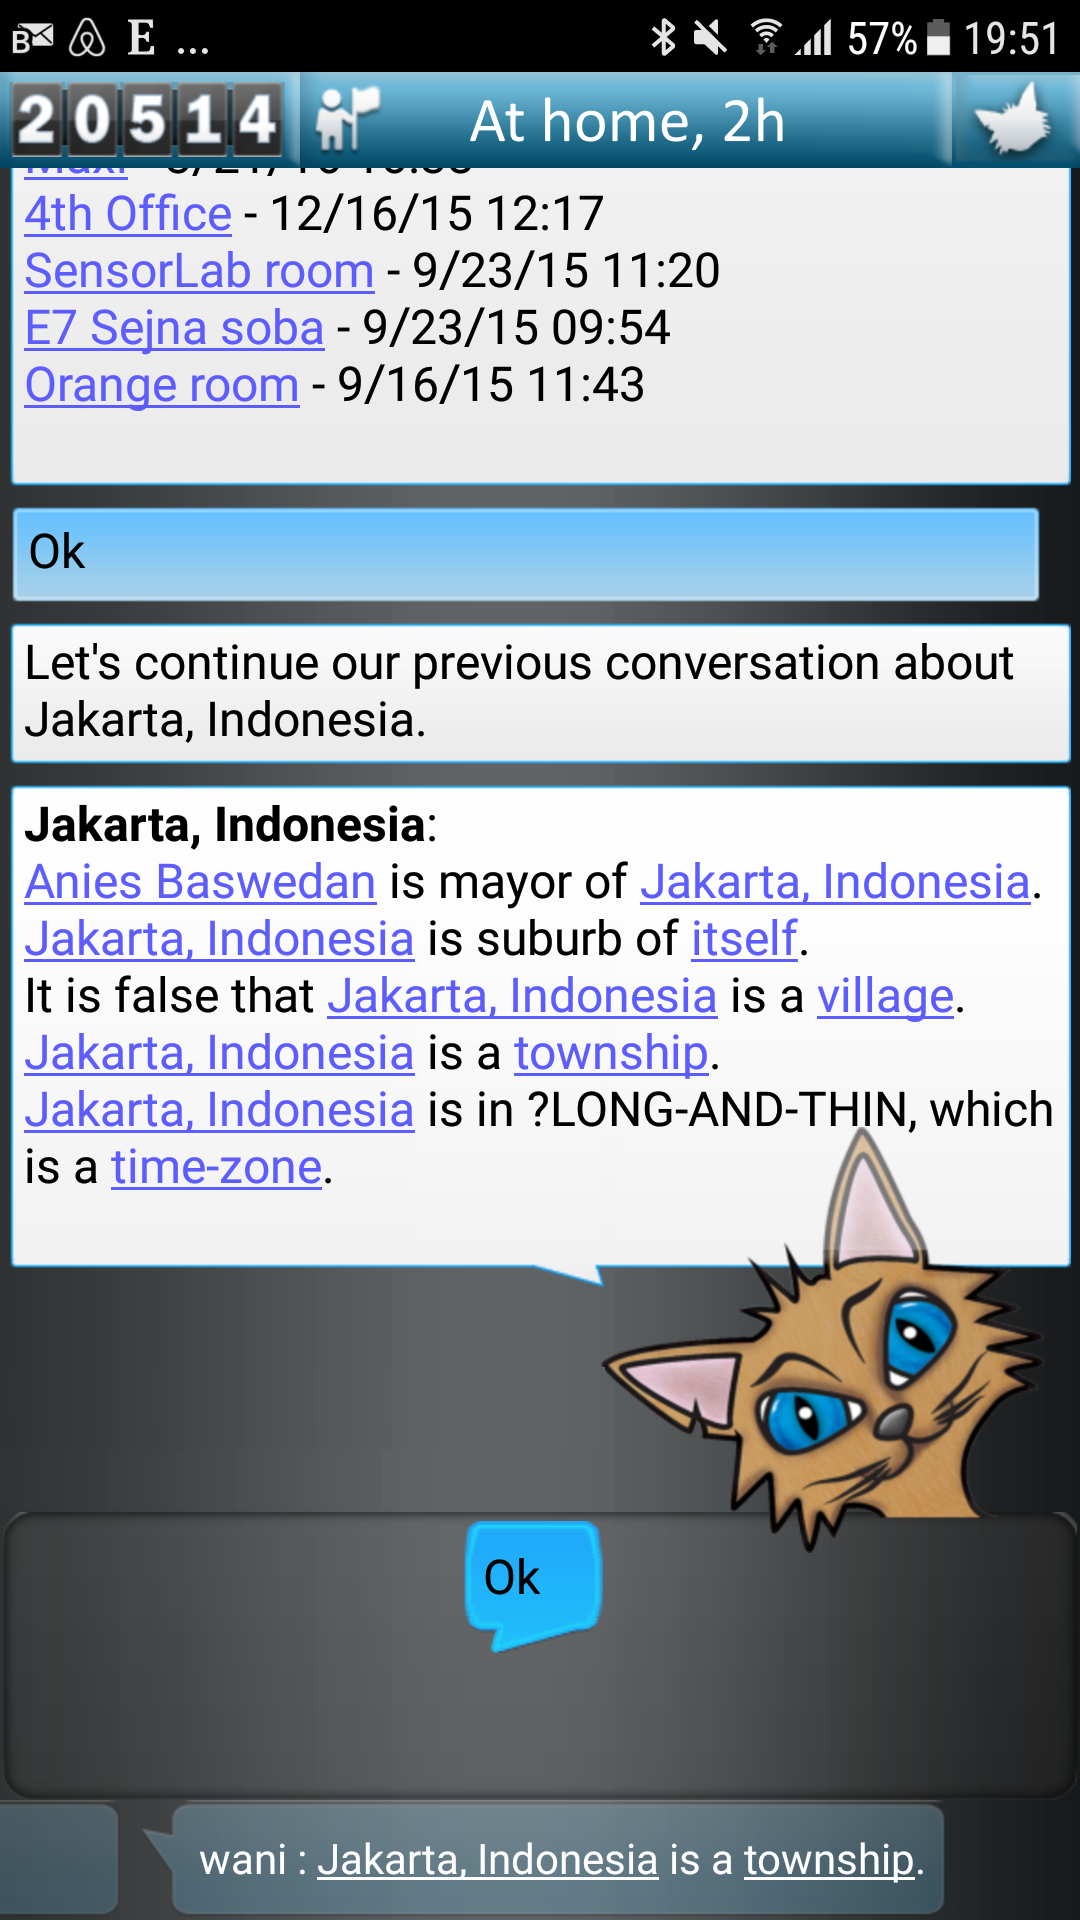
\includegraphics[width=0.41\textwidth]{figures/androidExample1.png}
	\caption{Screenshot of Curious Cat Android application.}
	\label{fig:androidExample}
\end{figure}

During this time, 5,185 users installed its
client app, out of which 2,401 users registered, and 1,715 users used it at 
least once (see the results chapter, \autoref{section:stickiness} for more 
details on users).
The development  of \emph{Curious Cat} implementation started on October 
26th, 2010 and halted on June 2014. The
implementation follows closely the architecture presented on 
\autoref{fig:Architecture} in \autoref{chapter:approach}. For the core
of the system we took Cyc with its common sense KB and inference engine, which 
was also an initial inspiration for the development and the approach, where
the main work needed to be done on the part of the meta-KB and also common
sense KB extensions to support our use-cases. For the NL modules, our 
implementation relies on the internal Cyc logic to NL conversion modules, and
on SCG\parencite{Schneider2015}. The procedural component and client were 
written from scratch. All together our implemented system consists of 50,686
lines of Java source code, and 12,616 lines of knowledge definitions (8,571) for
the additional knowledge we added in CycKB to drive our KA process.

Besides the implementation described here, this system was also implemented and
deployed as a real-time commuting companion\parencite{Figueiras2013}, and as an
RDF framework for on the field sensor information knowledge acquisition
\parencite{Bradesko2012a}. Commuting companion implementation and this 
implementation were also described in the books \emph{Intelligent Decision 
Technology Support in Practice}\parencite{Costa2016} and \emph{Handbook of Human 
Computation}\parencite{Witbrock2013}. This implementation was also mentioned
in the \emph{Communications of the ACM} magazine article\parencite{Geller2016}.

Implementation consists of Android based mobile client (see screenshot on
\autoref{fig:androidExample}), Java Servlet based
\emph{Procedural Component} with PostGreSQL database access, two Research 
Cyc instances 
(KB, Inference Engine, NL Conversion) to increase the speed and reliability 
of the system, \emph{Transcript Server} for syncing between Cyc instances, 
and a web-site for registration and email confirmation. This organization is 
also depicted on \autoref{fig:implementation} below.

\begin{figure}[H]
	\centering
		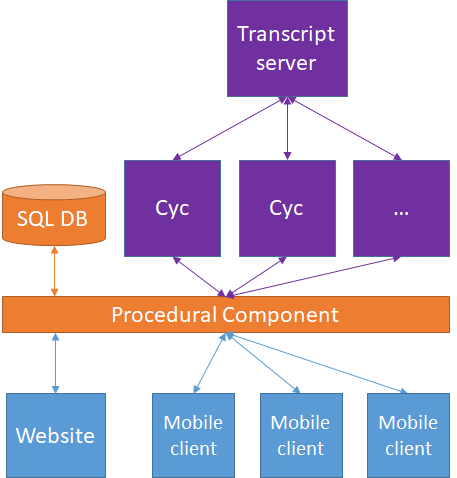
\includegraphics[width=0.62\textwidth]{figures/implementationOrg.png}
	\caption{Organization of the system modules in our implementation.}
	\label{fig:implementation}
\end{figure}

\section{Cyc}
\label{section:Cyc}
As already mentioned in related work (\autoref{section:relatedcyc}), \emph{Cyc}
is an AI project started in 1984 by Douglas Lenat\parencite{Lenat1985} with the
premise, that in order to make computers think like humans do, we need to first
make sure that they have same common sense knowledge as humans do. Since then,
\emph {Cyc} team (now part of \emph{Cycorp Inc.}), is codifying and entering 
the knowledge by hand and also by other means of knowledge acquisition and 
mining (see rows stating "Cyc" as parent in \autoref{tab:related}, 
\autoref{chapter:related} - \nameref{chapter:related}). 
The collected and codified knowledge is represented in machine-usable form 
using \emph{CycL (Cyc Language)}, and is structured and grouped together as
\emph{CycKB}. In parallel with the KB, Cyc also contains an inference engine
that works on the scale of the KB, and a set of tools, APIs and other interfaces
for interacting with the system, ranging from web interface, natural language,
web APIs and also Java interfaces, which we used in our implementation and
communication with the procedural part of our system 
(\autoref{section:prophet}).

%subsection
\subsection{Cyc KB}
\label{section:cyckb}
At this moment (end of 2017), \emph{Research CycKB} consists of more than 
630,000 concepts, 7,000,000 assertions (rules are also assertions), made with
using more than 38,000 predicates (relations), covering a broad domain of
human common sense knowledge. The KB is divided into thousands of micro-theories
(not counting the microtheories we added for \emph{CC} implementation - 
\autoref{section:crowdsourcing}), where each micro-theory is a set of assertions
that share common assumptions. Microtheories (Mts) can hierarchically stack on 
top of each other and allow \emph{Cyc} to independently maintain assertions that
could contradict each-other. This also enhances the performance of the 
\emph{Cyc} inference engine, since it can be limited on one particular, or a
group of Mts to limit the number of facts it needs to use while inferencing.

\emph{CycKB} is represented in \emph{CycL}, with most basic syntax described as:
\begin{itemize}
\item Logical constants are represented by "$\#\$$" sign, followed by the name 
of the term name ($\#\$JoesPizza$).
\item Formulas are enclosed in parenthesis. If more than one constants or terms
are part of the assertion, the predicate is always first, followed by its
arguments, for example: $(\#\$menuItem\quad\#\$JoesPizza\quad\#\$Pizza)$
\item Variables are represented by the question mark ("$?$") sign, followed
by the name in capital ($?PERSON$). For example, query asking the inference
engine, what is on the menu in Joe's Pizza is represented as: 
$(\#\$menuItem\quad\#\$JoesPizza\quad?ITEMS)$, where the name of the variable
"ITEMS", can be arbitrary.
\item Rules in \emph{CycKB} are represented by assertions using predicate 
$\#\$implies$, where the first argument is then it's antecedent and the second
argument a consequent (see CycL rule \ref{as:cycrule} below, which represents
the same upper ontology rule as defined in assertion 
\ref{rule:subclass_transitivity}).
\end{itemize}

Similar as with our example KB explaining CC approach, \emph{CycKB} is built on
top of upper ontology which gives it a formal grounding to support the rest of 
the KB. Our KA approach (\emph{Curious Cat} system) was implemented using 
\emph{Cyc}, and also inspired by its tool-set and unsolved problems. CC 
initially started as a solution for Cyc to speed up the NL based KA, so for our
explanations it was natural to pick and define an \emph{Upper Ontology} that 
can be easily mapped to \emph{CycKB}. While we cannot directly map all of the
definitions we used to explain the approach, we can map most of the Upper 
Ontology, which is given in the table below.

\begin{table}[h]
\centering
\caption{Mapping between upper ontologies of Cyc and our example KB constructed
to explain the approach.}
\label{tab:uppermap}
\begin{tabular}{|l|l|}
	\hline
	\textbf{CC Upper Concept} & \textbf{CycKB Upper Concept}\\
    \hline
    $is$ & $\#\$isa$ \\
    \hline
	$subclass$ & $\#\$genls$ \\
	\hline
	$arity$ & $\#\$arity$ \\
	\hline
	$argIs$ & $\#\$argIsa$ \\
	\hline
	$argClass$ & $\#\$argGenl$ \\
	\hline
	$Class$ & $\#\$Collection$ \\
	\hline
	$Predicate$ & $\#\$Predicate$ \\
	\hline
	$Something$ & $\#\$Thing$ \\
	\hline
	$Number$ & $\#\$NonNegativeInteger$\\
	\hline
\end{tabular}
\end{table}

Similarly as with constants, some rules can be mapped into Cyc versions by 
replacing implication form ($x \implies y$), with the CycL form 
($(\#\$implies\quad (x) \quad (y))$. For example, rule 
\ref{rule:subclass_transitivity} is in \emph{CycL} written as follows:
\begin{equation}\label{as:cycrule}
\begin{gathered}
\begin{aligned}
&(\#\$implies\\
	&\quad(\#\$and\\
		&\qquad(\#\$genls\quad?X\quad?Y)\\
		&\qquad(\#\$genls\quad?Y\quad?Z))\\
	&\quad(\#\$genls\quad?X\quad?Z))
\end{aligned}
\end{gathered}
\end{equation}

%subsubsection
\subsubsection{Curious Cat KB}
\label{section:cckb}
Even though \emph{CycKB} is one of the biggest and most complete common sense 
KBs that currently exist, it still does not cover everything and has missing 
knowledge. While it covers at least a bit of almost any topic within the general
knowledge, it often has missing parts that need to be extended in order to use
the knowledge in real world. While this is exactly what \emph{Curious Cat} is
helping to solve, we also added some of the knowledge by hand, to make initial
questions more interesting and to make it cover more topics. For the whole CC
implementation, we added an additional 8,571 assertions on top of the existing 
7mio assertions of \emph{CycKB} prior knowledge.
\begin{itemize}
\item New assertions are mostly KA meta-knowledge supporting the acquisition
mechanisms and logic.
\item Some of the new assertions are also missing general knowledge 
improvements on top of CycKB.
\end{itemize}

For the initial \emph{Cyc} knowledge entry process, we used ".ke" files, 
which support bulk import bigger amount of the assertions (see 
\autoref{fig:ketext}). After the system was already stable and running all the
time, this was replaced by the Transcript Server syncing as described below
in \autoref{section:transcriptserver}.

\begin{figure}[H]
	\centering
		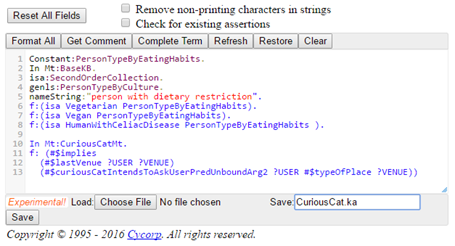
\includegraphics[width=0.9\textwidth]{figures/keEntry.png}
	\caption{Example screen of bulk importing assertions (knowledge) into Cyc.
This example is defining a concept $PersonTypeByEatingHabits$ and a rule 
generating questions about $typeOfPlace$ for last known user venue visit.}
	\label{fig:ketext}
\end{figure}

While mapping from our explanations to the actual \emph{Cyc} upper ontology is 
pretty straight forward since it is small, it would be impossible to describe
all details of more than 8,000 assertions that define the implementation of
CC KA approach. For example, the simple $ccWantsToAsk$ predicate (see
definition \ref{def:pred_ccWantsToAsk} \autoref{chapter:approach}, alternative 
in the real-world implementation
is 8 predicates (see definition \ref{as:cycCCAssertions} below), allowing us to
define much more complicated statements and
enriching them with possible suggestions as visible on \autoref{fig:ccmediated}.
Similarly, the KA rules are more complicated, using much bigger vocabulary
than we were able to explain. Example of one such rule is presented on
\autoref{fig:kaRuleImpl}.

On top of 7 million of preexisting \emph{Cyc} assertions and 8,571 of manually
added CC assertions, our system collected from users additional 524,276 
assertions (as of September 2017).

\begin{figure}[h]
	\centering
		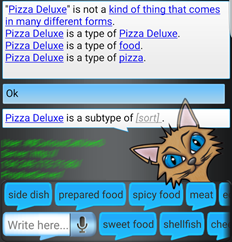
\includegraphics[width=0.4\textwidth]{figures/androidMediated.png}
	\caption{Example of human to computer interaction options generated with
$\#\$curiousCatIntendsToAskUserPredUnboundArg2WithChoices$.}
	\label{fig:ccmediated}
\end{figure}

\begin{figure}[h]
	\centering
		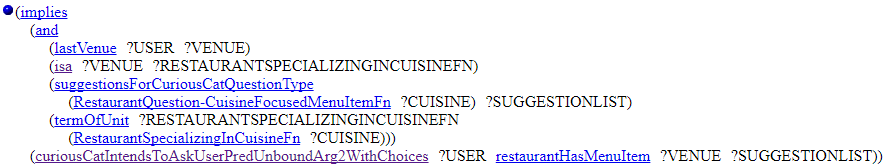
\includegraphics[width=1\textwidth]{figures/kaRule.png}
	\caption{Example of KA rule from CC implementation (screenshot from Cyc).}
	\label{fig:kaRuleImpl}
\end{figure}

\begin{equation}\label{as:cycCCAssertions}
\begin{gathered}
\begin{aligned}
&S_{CC Intents}=\{\\
&\quad\#\$curiousCatIntendsToAskUserPredBound,\\
&\quad\#\$curiousCatIntendsToAskUserPredUnboundArg2,\\
&\quad\#\$curiousCatIntendsToAskUserPredUnboundArg2WithChoices,\\
&\quad\#\$curiousCatIntendsToAskUserPredUnboundArg3WithChoices,\\
&\quad\#\$curiousCatIntendsToAskUserYesNoQuestionAboutVenue,\\
&\quad\#\$curiousCatIntendsToAskUserYesNoQuestionAboutVenueWithArgument,\\
&\quad\#\$curiousCatIntendsToAskWithChoices,\\
&\quad\#\$curiousCatWantsToAskUser\\
&\}
\end{aligned}
\end{gathered}
\end{equation}

%subsection
\subsection{Cyc Inference Engine}
\label{section:cycinference}
Cyc AI system also includes the inference engine which can work over the CycKB.
Because the KB is so big (more than 7 million assertions), approaches taken
by other inference engines (like RETE algorithm) does not scale well at this
size, while the included engine is with some tweaking still able to give 
results inside tolerable time frame. One of the techniques (mentioned before)
allowing this, is organization of the KB into micro-theories which allow the 
inference engine to reduce the size of the world it operates with at given
contexts.

Cyc Inference Engine is able to perform modus ponens and modus tollens 
inference, universal and existential quantification, and also mathematical 
calculations\footnote{http://www.cyc.com/subl-information/introduction-cyc-inferencing/overview-cyc-inferencing/}. The inference engine is constructed together
with a set of \emph{Inference Removal Modules} (each module is able to remove or
solve a specific problem from the inference problem). These modules can range
from very general, to very specific ones, registered to only solve problems
related to one particular logical predicate. For example, predicate 
$\#\$disjointWith$ can have a module that can tell whether the assertions using
this predicate are true or not (decides on disjointness). There are many
modules like this, implementing symmetry, transitivity and reflexivity, etc.

The engine is mostly controlled with rules (as for example the rule on 
\autoref{fig:kaRuleImpl}). The inference rules can be separated
into the forward and backward rules, which define whether they are to be used
by forward chaining or backward chaining while doing the inference. Forward
rules are triggered when something is asserted into the KB and then they produce
the results (assertions as defined in the consequent), while backward rules
are triggered when a logical query is being asked over the KB, and only support
the logic behind the answering, without actually physically populating the KB.
The example KA rule from the \autoref{fig:kaRuleImpl} is forward rule. 

Forward rules are causing the system to be slower when something is being added,
and also cause its memory consumption to increase (newly inferred assertions),
but on the other hand speed up the querying. Backward rules are the opposite,
not taking any burden on the system when the assertion is being added, but
trigger the inference which could be slow, when someone issues a query.

%subsection
\subsection{Cyc NL}
\label{section:cycnl}
In the \autoref{section:logicNL} and \autoref{section:NLLogic} we gave a 
simplest possible 
example of logic to NL and the opposite conversion, to explain and showcase the
approach taken by the \emph{Curious Cat}. While this served well for the
explanation, the implementation in real-world is inherently more complicated.
For the implementation we used Cyc logic to NL system which is part of 
\emph{Research Cyc}\autocite{Coppock2010,Baxter2005}, and is able to convert
a decent number of \emph{CycL} assertions into their natural language 
equivalents. In our example, we only used two (2) predicates to be able to
do that ($name$, $nlPattern$), but the implemented system uses more than
90 predicates and functions that are used to make the paraphrase system to work.
On the \autoref{fig:nlAssertion}, we can see the screenshot of
NL generation assertion using 4 paraphrase functions, unbound variables,
a string and a concept of the $Have-TheWord$. Then additionally, the concept
representing the word "have", has additional 79 language generation assertions
defining how to convert this word in various discourse contexts. 

\begin{figure}[h]
	\centering
		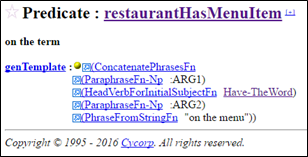
\includegraphics[width=0.6\textwidth]{figures/nlAssertion.png}
	\caption{Actual NL generation assertion example for the corresponding predicate for 
		$menuItem$ from our implementation (Cyc).}
	\label{fig:nlAssertion}
\end{figure}

As part of implementing \emph{CC}, we had
to extend this system and add multiple NL generating assertions to it, the
implementation is from \emph{Cyc AI System}, and is out of scope of this 
thesis. The details of this approach which can generate both referring 
expressions and non-referring expressions, including both referential and 
bound variable anaphora, are described in the paper written by
\textcite{Coppock2010}. 

To be able to convert from NL back to logic, our implementation also relies on
the functionality which is part of \emph{Cyc} and is described in more detail
in the Semantic Construction Grammar paper\parencite{Schneider2015}. The 
approach is similar as
taken by chat-bot engines\parencite{Wilcox2011}, which uses textual patterns
with special wild-cards, to map the actual text onto a predefined pattern, which
is then used to find a response. The difference is, that after the initial 
pattern matches are found, it uses \emph{CycL} mappings and then Inference 
Engine to check for
the formal validity of the resulting statements and consequently the parsing 
process. The other improvement is, that the the wild-cards in the patterns
can be typed (using Cyc constants). This means that that in such patterns, 
only terms of specific type can be fitted into a slot, which improves the 
conversion accuracy. An example pattern (taken from the paper) can be written 
like: "place[d|\{\}] \$ContainerArtifact\#0 over high heat".
During the years of CC experiment (as described in the 
\autoref{chapter:evaluation}), the logic to NL was used all the time (it is a
crucial component), while NL to logic was implemented but not always used, 
because it is more complex part of the software, harder to maintain, and was
also not of crucial importance for KA experiments.

%subsection
\section{Transcript Server}
\label{section:transcriptserver}
The \emph{Transcript Server} is an important technical part of the presented CC 
implementation, improving scalability, reducing downtime and also reducing
other maintenance costs. As visible in the implementation design 
(\autoref{fig:implementation}) sketch, it is a crowd based software module
to which all Cyc instances connect to. Software wise it is a simple database
server, which can receive and store for later, raw \emph{CycL} assertions 
(without any inference capabilities), and replicate them between 
connected \emph{Cyc} instances. Each of CC instances of \emph{Cyc} system is
set in a way, that after it wakes up, first syncs with the \emph{Transcript 
Server} and thus gets the knowledge added in the past. Besides the syncing,
it also forwards every new assertion to the \emph{Transcript Server} (if it was
not received from there). 

This simple mechanism allows us to have multiple \emph{Cyc} instances with
the same knowledge, which then allows simple load-balancing at query-time,
backup instances in cases when the main instance crashes. For the cases when
we had to manually shut down Cyc for upgrades or server maintenance, this simple
automatic syncing mechanism (even if being slow due to each assertion triggering
the inference engine again), saved us a lot of manual importing of the old knowledge.
 As of September 2017, full sync of CC collected knowledge (532,847 
assertions) takes approximately 2 days to finish.

%section
\section{Mobile Client}
\label{section:app}
The client part of the implemented KA approach is a simple Android application
(see screenshot on \autoref{fig:androidExample} at the beginning of the chapter).
The main screen consists of (listed top down as sections appear on the phone 
screen):
\begin{itemize}
\item Upper status bar, containing the points on the left, location info and 
button in the middle, ant a "cat" menu on the right.
\item Middle conversational section, where CC and user responses appear as
text in the conversational bubbles, similar to those that usually represent 
SMS messages. Each bubble can contain HTML formatted text, hyper-links and 
pictures.
\item Conversational section is followed by the "response section", where user
is presented with the set of possible responses, or a free text box. On the 
right of this GUI section, there is a cat's face, which acts as a button with
same functionalities as the "cat" menu on the upper right.
\item On the bottom, there is a swipe-able section, which contains contextual
bubbles representing what other users  who are nearby or are discussing same 
topics are answering.
\end{itemize} 

The logic behind the client is pretty straight forward. It is connected to the
\emph{Procedural Component} of CC system, which can send it a discourse object
containing a text which needs to be presented to the user, and some additional 
info such as ID of the statement, it's \emph{CycL} representation and also
suggestions for the user, and the points that user currently collected. When 
the user answers, this is sent back to the server, together with the ID of the 
discourse. In the cases, when the server wants to pro-actively ask something,
and the phone is in a sleep mode (meaning that the pro-activity didn't occur due
to location change), it can generate a \emph{Firebase Cloud Messaging (FCM)}
message with the same object as
it would send directly, and then this is presented to the user when he/she 
looks at the phone.

Additionally to this answer/reply functionality, represented as blue arrows on
\autoref{fig:Architecture}, the client keeps a back-channel with the 
server's \emph{Procedural Component}, and is periodically sending a location,
local time and language. In order to not consume a lot of the battery, the 
client is mostly sleeping, and only wakes up every 3min and tries to get a GPS
signal for 20 seconds. If the signal is too low and cannot acquire accurate 
enough location in 20 seconds, it stops trying and goes back to sleep mode.
The back-channel is also opened each time user opens the client application
manually.

%section
\section{Procedural Component}
\label{section:prophet}
This component serves as the main interface between the \emph{CC} system and
the external world, and as a glue, keeping all the parts of the system in sync
and together as a coherent KA platform. This component consists of a database,
two Java servlets, and a separate Node.js server handling the geo-spatial 
context mining functions. Each of the servlets is handling one type of 
interaction with the client applications:
\begin{itemize}
\item \emph{Main Interaction Servlet} is taking care of the user sessions, and 
main interaction loop between the user and the system. This servlet is handling
most of the work when user is receiving and answering the questions. It also
asserts and detects new topics, when user clicks hyper-linked concepts that
are presented as part of the conversational bubbles.
\item \emph{Location Servlet} is accepting GPS records from the phone, calling
the geo-spatial clustering service and then asserting current location and 
time assertions into \emph{Cyc}, as described in \autoref{section:context}.
Additionally, this servlet is providing the contextual clues (bubbles at the
bottom of Android app. as visible on \autoref{fig:androidExample}) to the 
clients.
\end{itemize}

%subsection
\subsection{Main Interaction Servlet}
\label{section:mainServlet}
When this component gets the request from the client, it first checks whether
it is linked to one of the statement IDs that were sent to the client. This
identifies, whether this is an answer to some previous questions that CC
asked, or is a completely new discourse. This identification can be done on 
the client already, since the GUI is constructed in a way, that it is obvious
to the user, he is answering a question. If he wants to do something completely
independent, the guided mechanism "forces" the user to click on 
"something else", where he can then start a completely new discourse.
After this is identified, the system asserts into  \emph{Cyc} and logs
in the database  the time of last user response, and text of the
response. After this, depending on whether it was identified as an answer to
previous question, or a completely new discourse (statement, question), it goes
into the \emph{Consistency Check and KB Placement} mode 
(\autoref{section:consistency}), or \emph{NL to Logic} mode 
(\autoref{section:NLLogic}), as described in the appropriate sections in the 
\autoref{chapter:approach}. 

After this step, when the system already remembered
the user answer, or understood user query, this servlet asks \emph{Cyc} for
new questions and comments that \emph{Curious Cat/Cyc} might have. This is done
with logical queries like this (let's say that the current user is $User1$):
$(curiousCatWantsToAskUser\quad User1 \quad ?QUESTION \quad ?SUGGESTIONS)$. This
will then cause he inference engine to search through all the assertions and
trigger all the backward rules in the micro-theory KB of $User1$, and come up
with the answers, filling the variables $?QUESTION$ and $?SUGGESTIONS$. The list
of questions (given in logic, \emph{CycL}) is then analyzed by the servlet,
which picks the first one that was not there before (on previous interaction),
and mentions the concept that is set as a current topic. Topics are organized
into a stack, where the concepts user is mentioning when answering questions
about the current topic, are constantly being added on top of the stack 
(\autoref{tab:topics}). 
In addition to these "user caused" topics, stack contains a three predefined
topics at the bottom. First one (last to be used - at the bottom), is a
random topic that gets chosen by the system. Second "topic" is actually a
question, whether there is some particular topic that would interest the user.
The third one (first of the system's topics, to be used when it runs out of
the questions), is the concept of the user itself. If it happens that \emph{CC}
runs out of other topics, it starts discussing about the user. 

\begin{table}[h]
\centering
\caption{Stack of conversational topics.}
\label{tab:topics}
\begin{tabular}{|c|}
	\hline
	\textbf{$\#\$CurrentTopic$}\\
    \hline
	\hline
    $\vdots$  \\
    \hline
	$\#\$AnswerConcept2$ \\
	\hline
	$\#\$AnswerConcept1$ \\
	\hline
	$\#\$PreviousTopic$ \\
	\hline
	$\#\$PreviousConcept1$ \\
	\hline
	$\#\$UserConcept$ \\
	\hline
	$\#\$AskUserForTopic$ \\
	\hline
	$\#\$Random$ \\
	\hline
\end{tabular}
\end{table}

For example, in \autoref{tab:topics}, we can see that the current topic is
taken out of the stack (separated by the double line), and the other concepts 
that were in the answers of the questions, were added on top 
($\#\$AnswerConcept2$). We can also see, that the topics are added back on the
stack, if their questions are not depleted yet (as happened for the 
$\#\$PreviousTopic$). For example, let's say that the $\#\$PreviousTopic$ was
\emph{Joe's pizza} restaurant, which was on the stack right above the 
$\#\$UserConcept$ topic. It was taken out of stack, and then when user answers
the first question (let's say "they have pizzas on the menu" as in our other
examples), concept $\#\$PreviousConcept1$ represent $\#\$Pizza$, and is added
on the stack. Then user decides that she wants to discuss about some other 
topic ($\#\$CurrentTopic$), and this causes the $\#\$PreviousTopic$ to be put
back on the stack, since not all questions were depleted. But now, it sits
on top of the "Pizza" topic ($\#\$PreviousConcept1$). The $\$\#AnswerConcept1$ 
and $\#\$AnswerConcept2$ were then added on top of the stack, as a consequence 
of answering questions inside the $\#\$CurrentTopic$ topic. An additional 
fail-back mechanism (not presented on \autoref{tab:topics}), for when the
topic is depleted of the KA questions, is to call internal \emph{Cyc CURE} API
\autocite{Witbrock2010}, to get a list of general, or internal \emph{Cyc} 
questions (not using any context) that could be asked for particular concept.

%subsecton
\subsection{Location Servlet}
\label{section:locationServlet}
When the client sends the GPS location and user local time (either when 
periodically waking up, or when user turns on the application), the coordinate
gets into a clustering algorithm which detects whether this is part of user
moving between the locations, or is part of the visit of particular location.
In the case, when user is moving, this is asserted into \emph{Cyc} as the user
activity, but no particular action is taken. This simply influences the 
\emph{CC} responses in cases, when user interacts with the system while he is
on the way. On the other side, when the algorithm detects that user is at 
particular location, this goes to the second algorithm, which checks online 
APIs(Factual, Foursquare) for the type and name of the place. This information,
together with the time of arrival and current stay, is asserted into \emph{Cyc},
together with the new topic, representing the concept of the new location. 
At this point the system "knows" the user is staying at particular place and 
might have some free time, even if the client application is sleeping, it sends
a FCM message with a new contextual questions, which appears as a notification
on the user's phone.

The first part of the clustering algorithm is an improved implementation of
already mentioned (\autoref{section:SPD1} in \autoref{chapter:related} and
described in \autoref{section:minedContext} in \autoref{chapter:approach})
SPD (Staypoint Detection) algorithm\parencite{Kang2005}. Our improvements
and extension to the algorithm\parencite{Kazic2017} improved the accuracy and 
robustness by a
large factor\footnote{An additional paper with the full explanation and 
evaluation of 
extended SPD algorithm that can be used in any location-based application is 
in preparation}, and can be quickly summarized:
\begin{itemize}
\item Removing some unnecessary steps performed in the original algorithm (step
13 from the paper written by \textcite{Kang2005}.
\item Extending the algorithm to also reports locations that are not detected
as a point of stay and thus allow it to be an online algorithm, working in
real-time, quickly responding to possible location changes and reporting 
whether the user is currently traveling or at a fixed location. This is achieved
by keeping the index of locations, until completely clustered. The paths
are then locations from this index, not included in any of the clusters. 
Additionally, the current cluster (marked as $CL$ on the \autoref{alg:spd1}),
is returned each time as well, marked as unfinished.
\item Adding an optional second iteration of the algorithm which fine tunes
promising detected stay-points from the first iteration. This cleans the 
potential errors, when one or a few raw GPS locations jumped outside the 
perimeter but then the sensor stabilizes. This adds another loop through
the detected clusters at the end of each iteration. It creates one visit
(stay-point) on the occasions when the path between two same locations lasts 
less than a given threshold, which is the most common mistake appearing in the
results of the original algorithm.
\item Adding an additional analytics steps, including enrichment of the detected
stay-points and predicting user's next destinations.
\end{itemize}

This algorithm through the years while \emph{CC} is online evolved from a few
"if" statements running locally on the phone, to a separate service and mobile
library serving also other projects, due to it's general usefulness for 
geo-spatial analytics. The data that the clients (not just \emph{Curious Cat}
are sending and the service is analyzing, can be visualized and browsed through
a separate web-interface as visible on \autoref{fig:nextPin}.

\begin{figure}[htb]
	\centering
		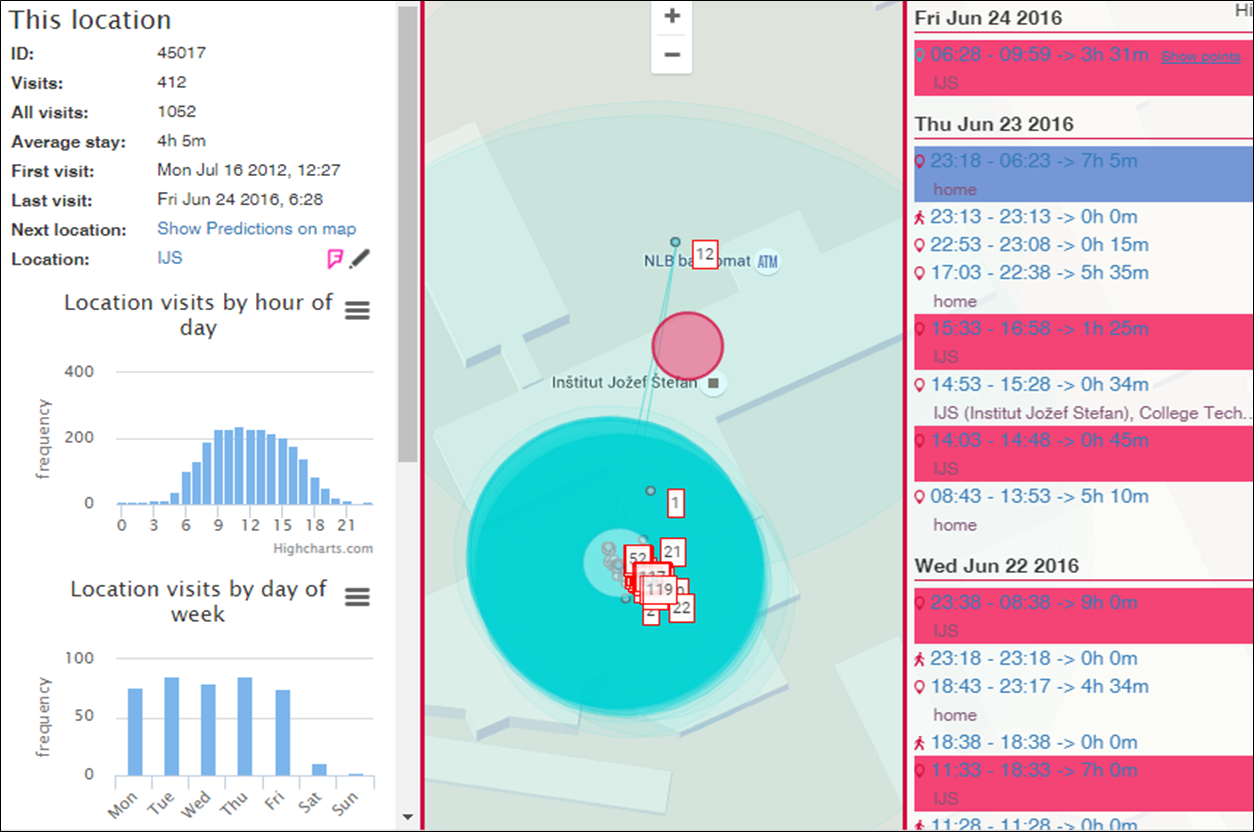
\includegraphics[width=1\textwidth]{figures/nextPin.png}
	\caption{Visualization of clustering and enrichment results the SPD
algorithm, to provide $probableUserLocation$ context.}
	\label{fig:nextPin}
\end{figure}

The second part of this algorithm was inspired by the paper \emph{Applying 
Commonsense Reasoning to Place Identification}\parencite{Mamei2010}, which
probabilistically ranks the possible places acquired from online APIs based on the
SPD results and current time of the day. This then additionally enriches (with
the name and type of the place) raw geo-coordinates of the cluster and time 
as given by the SPD algorithm alone. 

Additionally to handling user current location and time, 
\emph{Location Servlet} also uses this context, together with the current topic
(\autoref{tab:topics}), to query for latest non-private answers from other
users that are nearby, or talking about the same concepts as our example user.
This is represented by contextual clues at the bottom of the client application
(\autoref{fig:androidExample}).

%section
\section{Assisting and Using Gained Knowledge}
\label{section:usage}

One of the main ideas behind the proposed KA approach, is to be able to
incorporate
it into some other activity, and do the KA unobtrusively and cheaply as a side
effect of the main purpose of the software. This was also our initial aim when
we started the \emph{Cyc} based implementation of proposed KA system. The end 
goal of the KA is thus not the KA itself, but to be able to collect good 
enough knowledge to be able to use by the inference to solve some higher-level 
tasks previously not possible. To prove this concept, we added a few inference 
rules which try to combine all the gained knowledge to produce relevant 
suggestions when user requests them, or when the system thinks the user is 
hungry (no eating reported for a while). Additionally, the system is able to 
infer, based on the events around the user and his likes (answered questions 
about what user likes).

\begin{figure}[htb]
	\centering
		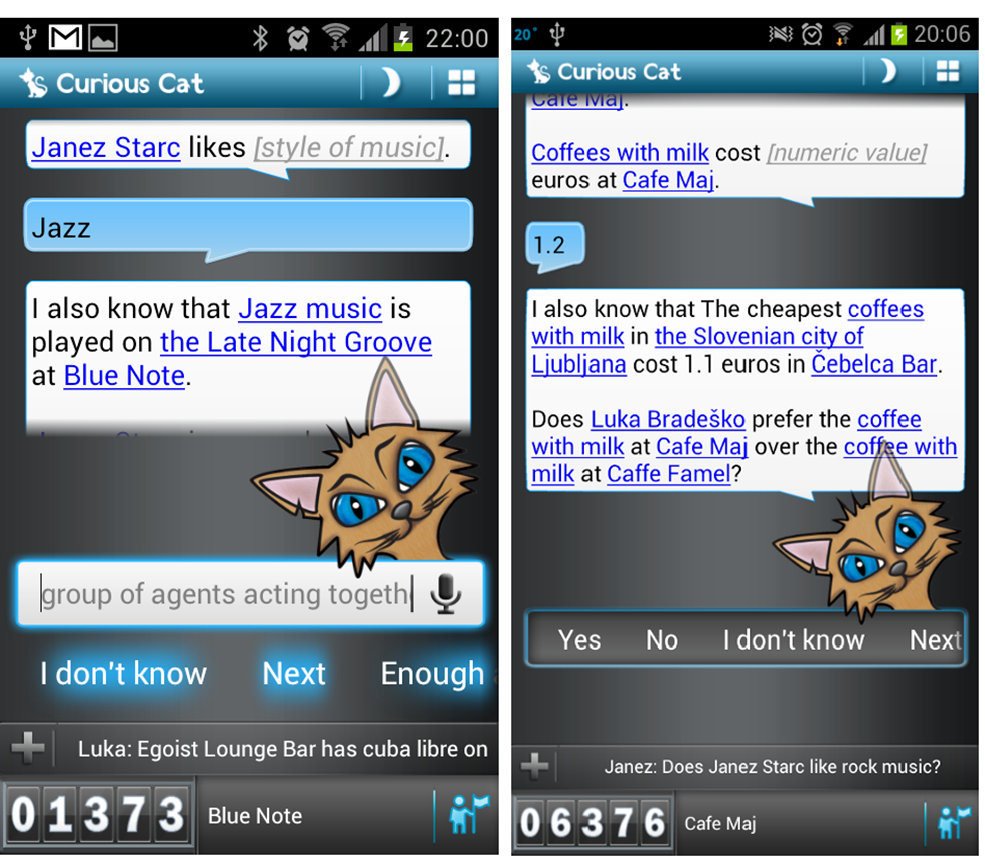
\includegraphics[width=0.8\textwidth]{figures/assistExample1.png}
	\caption{Example suggestions for a live music (after it learns that the user likes jazz), and information that there is a cheaper coffee nearby, followed by the comparison question to be able to suggest better in the future}
	\label{fig:assist1}
\end{figure}

On the left screenshot of \autoref{fig:assist1}, we see that \emph{Curious Cat}
smartly told the user that there is a (jazz) music event nearby, after it 
learned that the user likes jazz music. The event was actually entered by 
another user and the system picked it up from the KB for the purpose of 
helping new user. On the right screenshot, there is a similar ad-hoc comment, 
but this time the trigger was cheaper coffee in the bar next-door. The 
suggestion is immediately followed by the comparison question, to be able to 
better rank the coffees next time.

A more complex inference suggestion when user asked for something fast to eat 
is presented on the \autoref{fig:assist2}. There the inference engine combined 
multiple pieces of knowledge:
\begin{enumerate}
\item Hot horse serves fast food cuisines, therefore it must be a fast food 
restaurant
\item User likes fried food
\item French fries are a type of fried food
\item Hot Horse has French fries on the menu
\item Since Hot Horse is a fast food restaurant which is near the user, and has 
something on the menu that the user likes, it is among the good suggestions.
\end{enumerate}

\begin{figure}[htb]
	\centering
		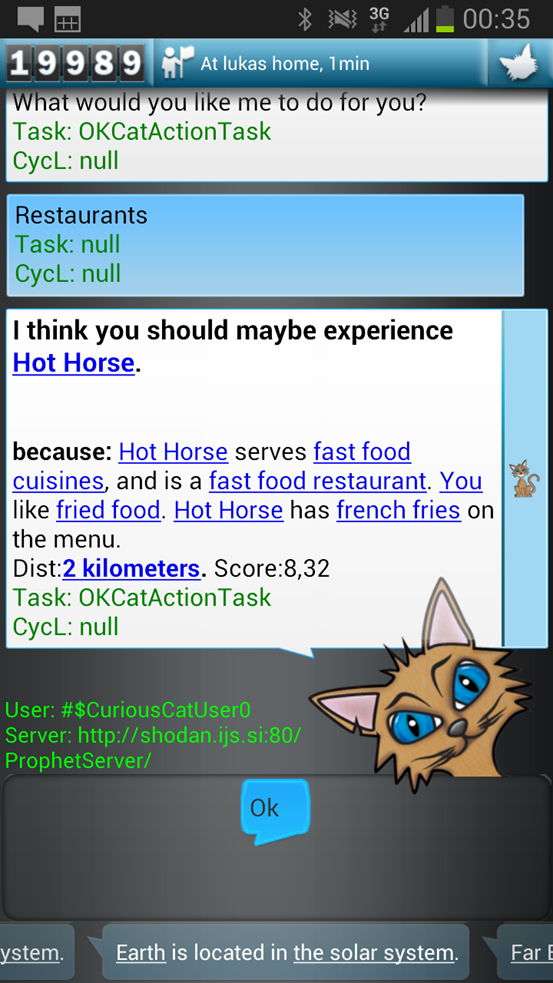
\includegraphics[width=0.4\textwidth]{figures/assistExample2.png}
	\caption{Suggestion as a complex inference result combining knowledge about cuisines, user likes and place specifics.}
	\label{fig:assist2}
\end{figure}

This inference process was then structured into the set of logical statements 
(special inference rule for suggestions), sent through the NL conversion  and 
presented to the user as the suggestion text. 
While this suggestion is a simple basic example, still shows the power of 
combining separate piece of logic by inference and produce some useful results. 
The step from liking the fried food to French fries on the menu would be quite 
hard to tackle with standard approaches, especially if we consider it just an 
example of a general mechanism.

